% Created 2022-05-04 Wed 15:46
% Intended LaTeX compiler: xelatex
\documentclass[lang=cn]{elegantbook}
                 \usepackage{minted}
                 \usepackage{xeCJK}
\setCJKmainfont{LXGW WenKai}
\documentclass[pad]{elegantbook}
\documentclass[hang]{elegantbook}
\author{Mushi}
\date{\textit{[2022-04-30 Sat 16:27]}}
\title{C++ Primer Note}
\hypersetup{
 pdfauthor={Mushi},
 pdftitle={C++ Primer Note},
 pdfkeywords={},
 pdfsubject={},
 pdfcreator={Emacs 27.2 (Org mode 9.6)}, 
 pdflang={English}}
\begin{document}

\maketitle
\tableofcontents



\mainmatter

\chapter{开始}
\label{sec:org336a5d8}

\begin{introduction}
  \item 一个简单的 C++ 程序
  \item 输入输出
  \item 注释简介
  \item 控制流
  \item 类简介
  \item 书店程序
\end{introduction}

\section{编写一个简单的 C++ 程序}
\label{sec:orgea8268a}

每个 C++ 程序都包含一个或多个 \textbf{函数} (function), 其中一个必须命名为 \texttt{main}. 操作系统
通过调用 \texttt{main} 来运行 C++ 程序.

\vspace*{1\baselineskip}

示例如下所示:

\begin{minted}[]{cpp}
int main() {
  return 0;
}
\end{minted}

一个函数的定义包含四部分: \textbf{返回类型} (return type), \textbf{函数名} (function), 一个括
号包围的 \textbf{形参列表} (parameter list, 允许为空) 以及 \textbf{函数体} (function body)

\texttt{main} 函数的返回类型必须是 \texttt{int}, 即整数类型. \texttt{int} 类型是一种 \textbf{内置类型}
(built-in-type), 即语言自身定义的类型.

这个语句中唯一的一条语句是 \texttt{return}, 它结束函数的执行. 在本例中, \texttt{return} 还会向
调用者返回一个值. 当 \texttt{return} 语句包括一个值时, 次返回的类型必须与函数的返回类型
相容.

\vspace*{1\baselineskip}

\begin{note}
在 C/C++ 中, 新手常犯的错误就是忘记写分号. 代码写多了形成条件反射了就好了(当然有时候还是会漏掉 LOL).
\end{note}

\vspace*{1\baselineskip}

在大多数系统中, \texttt{main} 的返回值被用来指示状态. 返回值 \texttt{0} 表示成功. 非 \texttt{0} 返回
值由系统定义, 通常用来指出错误类型.

\vspace*{1\baselineskip}

\begin{definition}[类型]
类型是程序设计中最基本的概念之一, 在本书中我们会反复遇到他. 一种类型不仅定义了数据元素的内容, 还定义了这类数据上可以进行的运算.

程序所处理的数据都保存在变量中, 而每个变量都有自己的类型.
\end{definition}

\subsection{编译, 运行程序}
\label{sec:orgcde4eb9}

如何编译程序依赖于你使用的操作系统和编译器. 这里我不想展开讨论, 你可以通过搜索引
擎解决这些问题. 你的搜索关键词应该是 ``<你的操作系统> + 搭建 C++ 运行环境''

尽管在生产环境中使用 \textbf{集成开发环境} (Integrated Developed Enveloped Environment,
IDE) 是高效的. 但我个人还是推荐你先借助命令行界面学习 C++ 本身, 一旦你掌握了语言,
IDE 再强大也只是一个工具而已.

\begin{enumerate}
\item 程序源文件
\label{sec:org41a80d5}

大多数编译器都要求程序源码存储在一个或多个文件中. 程序文件通常被称为 \texttt{源文件}
(source file).

不同编译器使用不同的后缀命名方式, 最常见的包括 \texttt{.cc}, \texttt{.cxx}, \texttt{.cpp}, \texttt{.cp} 及 \texttt{.c}

\item 从命令行运行编译器
\label{sec:org15e4064}

这里我简单演示一下命令行编译过程, 见下图:

\begin{center}
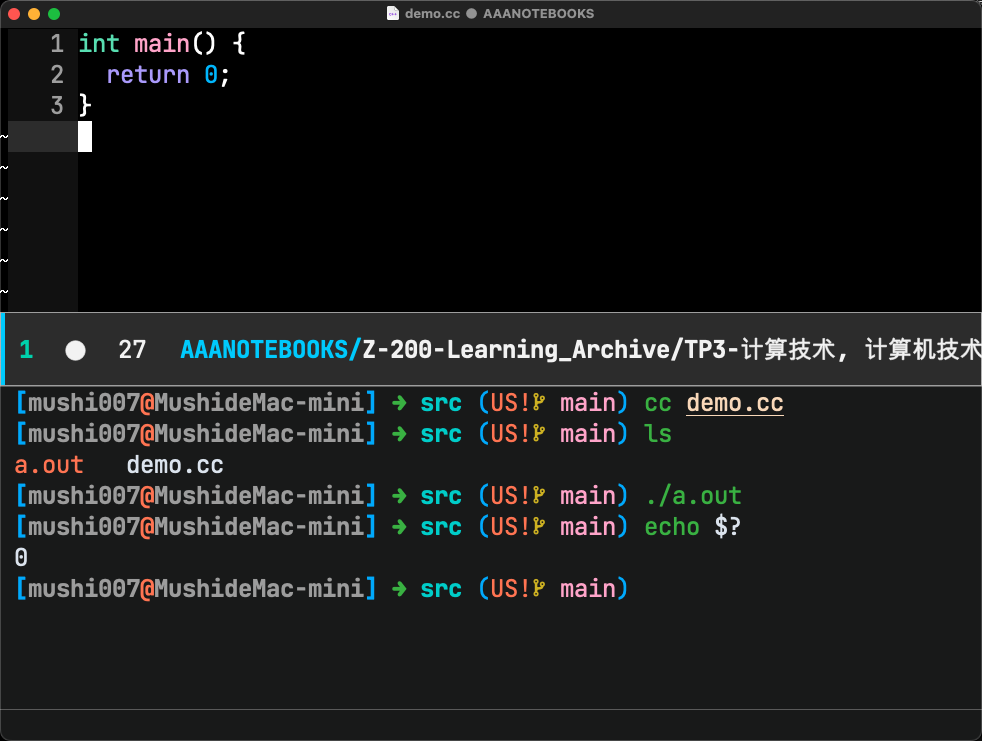
\includegraphics[width=1.0\textwidth]{img/democc_演示.png}
\end{center}

\begin{note}
这里的 echo \$? 是一个 UNIX 命令, 它这里返回的就是最近的函数返回值. 在 Windows 系统中, 可以键入 echo \%ERRORLEVEL\% 查看
\end{note}
\end{enumerate}

\section{初始输入输出}
\label{sec:org9122157}

C++ 语言并未定义任何输入输出 (IO) 语句, 取而代之, 包含了一个全面的 \textbf{标准库}
(standard library) 来提供 IO 机制 (以及很多其他设施).

\textbf{iostream} 库包含两个基本类型 \textbf{istream} 和 \textbf{ostream}, 分别表示输入流和输出流. 一
个流就是一个字符序列. 术语 (stream) 想要表达的是, 随着时间的推移, 字符是顺序生
成或消耗的.

\subsection{标准输入输出对象}
\label{sec:orge52d0bb}

标准库定义了 4 个 IO 对象, 见下表:

\begin{table}[htbp]
\label{4 个 IO 对象}
\centering
\begin{tabular}{llll}
对象名 & 作用 & 别称 & 所属类\\
\hline
\texttt{cin} & 处理输入 & 标准输入 (standard input) & \texttt{istream}\\
\texttt{cout} & 处理输出 & 标准输出 (standard output) & \texttt{ostream}\\
\texttt{cerr} & 输出警告和错误消息 & 标准错误 (standard error) & \texttt{ostream}\\
\texttt{clog} & 输出程序运行时的一般性信息 & 无 & \texttt{ostream}\\
\end{tabular}
\end{table}

系统通常将程序所运行的窗口与这些对象关联起来. 因此, 当我们读取 \texttt{cin}, 数据将从程
序正在运行的窗口读入, 当我们向 \texttt{cout}, \texttt{cerr}, 和 \texttt{clog} 写入数据时, 将会写到同
一个窗口.

\subsection{一个使用 IO 库的程序}
\label{sec:orga776e5c}

在书店程序中, 我们需要将多条记录合并成单一的汇总表. 作为一个相关的, 但更简单的问
题, 我们先看一下如何将两个数相加. 通过使用 IO 库, 我们可以拓展 \texttt{main} 程序, 使之
能提示用户输入两个数, 然后输出它们的和:

\begin{minted}[]{cpp}
#include <iostream>

int main() {
  std::cout << "Enter two numbers:" << std::endl;
  int v1 = 0, v2 = 0;
  std::cin >> v1 >> v2;
  std::cout << "The sum of " << v1 << " and " << v2
            << " is " << v1 + v2 << std::endl;
  return 0;
}
\end{minted}

尖括号中的 \texttt{iostream} 指出了一个 \texttt{头文件} (header). 我们一般一个程序的所有
\texttt{\#include} 指令都放在源文件的开始位置.

\subsection{向流写入数据}
\label{sec:orgab98561}

\texttt{main} 函数体的第一条语句执行了一个 \textbf{表达式} (expression). 在 C++ 中, 一个表达式
产生一个计算结果, 它由一个或多个运算对象和 (通常是) 一个运算符组成.

这条语句使用了 \textbf{输出运算符} (\texttt{<<}) 在标准输出上打印消息:

\begin{minted}[]{cpp}
std::cout << "Enter two numbers:" << std::endl;
\end{minted}

\texttt{<<} 运算符接受两个运算对象: 左侧的运算对象必须是一个 \texttt{ostream} 对象, 右侧的运算
对象是要打印的值. 此运算符将给定的值写到给定的 \texttt{ostream} 对象中. 计算结果是我们
写入给定值的那个 \texttt{ostream} 对象.

我们的输出语句使用了两次 << 运算符. 我们的表达式等价于:

\begin{minted}[]{cpp}
(std::cout << "Enter two numbers:") << std::endl;
\end{minted}

我们也可以把它变成两条语句, 效果是一样的:

\begin{minted}[]{cpp}
std::cout << "Enter two numbers:";
std::cout << std::endl;
\end{minted}

第一个输出运算符给用户打印一条消息. 这个消息是一个 \textbf{字符串字面值常量} (string
literal).

第二个运算符打印 \texttt{endl}, 这是一个被称为 \textbf{操纵符} 的特殊值. 写入 \texttt{endl} 的效果是
结束当前行, 并将与设备关联的 \textbf{缓冲区} (buffer) 中的内容刷到设备中.

\vspace*{1\baselineskip}
\begin{note}
程序员常常在调试时添加打印语句. 这类语句应该保证 "一直" 刷新流. 否则, 如果程序崩溃, 输出可能还留在缓冲区中, 从而导致关于程序崩溃的错误推断.
\end{note}

\subsection{使用标准库中的名字}
\label{sec:orgf8d9bd6}

前缀 \texttt{std::} 指出名字 \texttt{cout} 和 \texttt{endl} 是定义在名为 \textbf{std} 的命名空间 (namespace)
中的. 命名空间可以避免名字定义的冲突, 标准库定义的名字都在命名空间 \texttt{std} 中.

当我们使用标准库中的一个名字时, 必须显示说明我们想使用来自命名空间 \texttt{std} 中的名
字. 例如, 需要写出 \texttt{std::cout}, 通过使用 \textbf{作用域运算符} (\texttt{::}) 来指出我们想使用
定义在命名空间 \texttt{std} 中的名字 \texttt{cout}. 后面我们会介绍一种更简单的访问命名空间的方
法.

\subsection{从流读取数据}
\label{sec:org6d86399}

\begin{minted}[]{cpp}
int v1 = 0, v2 = 0;
\end{minted}

我们将这两个变量定义为 \texttt{int} 类型, \texttt{int} 是一种内置类型, 用来表示整数. 还将它们
\textbf{初始化} (initialize) 为 0. 初始化一个变量, 就是在变量创建的同时为它赋予一个值.

下一条语句是

std::cin >> v1 >> v2;

\textbf{输入运算符} (\texttt{>>}) 与输出运算符相似

\subsection{完成程序}
\label{sec:org7232608}

剩下的就是打印计算结果了:

\begin{minted}[]{cpp}
std::cout << "The sum of " << v1 << " and " << v2
          << " is " << v1 + v2 << std::endl;
\end{minted}

可以发现, 这里的运算对象并不都是相同类型的值. 某些运算对象是字符串字面值常量, 某
些是 \texttt{int} 值.

标准库定义了不同版本的输入输出运算符, 来处理这些不同类型的运算对象.

\section{注释简介}
\label{sec:org3af03d5}

注释可以帮助人类读者理解程序.

\subsection{C++ 中的两种注释}
\label{sec:orgd39aca4}

\begin{minted}[]{cpp}
// 双斜线注释常用于半行和单行附注.

/* 注释界定符
   通常用于
   多行注释
*/
\end{minted}

\subsection{注释界定符不能嵌套}
\label{sec:org1097362}

界定注释符不能嵌套使用, 如果你这么做了, 编译器会产生错误.

最好的方式是用双斜线注释掉代码段的每一行.

\begin{minted}[]{cpp}
// /*
// * 单行注释中的任何内容都会被忽略
// * 包括嵌套的注释对也一样会被忽略
// */
\end{minted}

\section{控制流}
\label{sec:orgcaf50fa}

语句一般是顺序执行的, 但程序设计语言提供了多种不同的控制流语句, 允许我们写出更为
复杂的执行路径.

\subsection{while 语句}
\label{sec:org3ec64c5}

\textbf{while语句} 反复执行一段代码, 直到给定条件为假为止. 我们可以用 \texttt{while} 语句编写
一段程序, 求 1 到 10 这 10 个数的之和:

\begin{minted}[]{cpp}
#include <iostream>
int main() {
  int sum = 0, val = 1;
  // 只要 val 的值小于等于 10, while 循环就会持续执行
  while (val <= 10) {
    sum += val; // 将 sum + val 赋予 sum
    ++val;      // 将 val 加 1
  }
  std::cout << "sum of 1 to 10 inclusive is "
            << sum << std::endl;
  return 0;
}
\end{minted}

我们编译这个程序, 它会打印出:

\begin{verbatim}
sum of 1 to 10 inclusive is 55
\end{verbatim}


\texttt{while} 语句的形式为:

\begin{minted}[]{cpp}
while (condition)
  statement
\end{minted}

\texttt{while} 语句的执行过程就是交替地监测 condition 条件和执行关联的语句 statement,
直至 consition 为假时停止. 所谓 \textbf{条件} (condition) 就是一个产生真或假的结果的表
达式.

条件中使用了 \textbf{小于等于运算符} (<=) 运算符来比较 val 的当前值和 10.

循环体是由两条语句组成的语句块.

\begin{minted}[]{cpp}
{
    sum += val; // 将 sum + val 赋予 sum
    ++val;      // 将 val 加 1
}
\end{minted}

所谓 \textbf{语句块} (block) 就是用花括号包围的零条或多条语句的序列. 语句块也是语句的一
种, 在任何要求使用语句的地方都可以使用语句块.

上面的语句块的第一条语句使用了 \textbf{复合赋值运算符} (+=). 此运算符将其右侧的运算对象
加到左侧运算对象中. 它本质上与一个加法结合一个 \textbf{赋值} (assignment) 是相同的.

第二条语句使用 \textbf{前缀递增运算符} (++). 递增运算符将运算对象的值增加 1. \texttt{++val} 等
价于 \texttt{val=val+1}.

\subsection{for 语句}
\label{sec:orge2d2ae3}

在 \texttt{while} 语句中, 使用变量 \texttt{val} 来控制循环执行的次数. 在循环条件中监测 \texttt{val} 的
值, 在 \texttt{while} 循环体中将 \texttt{val} 递增.

这种在循环条件中检测变量, 在循环体中递增变量的模式使用非常频繁, 以至于 C++ 语言
专门定义了第二种循环语句, \textbf{for 语句}, 来简化复合这种模式的语句. 可以用 \texttt{for} 语
句来重写从 1 加到 10 的程序:

\begin{minted}[]{cpp}
#include <iostream>
int main() {
  int sum = 0;
  // 从 1 加到 10
  for (int val = 1; val <= 10; ++val) {
    sum +=val;
  }
  std::cout << "Sum of 1 to 10 inclusive is "
            << sum << std::endl;
  return 0;
}
\end{minted}

每个 \texttt{for} 语句都包含两部分: 循环头和循环体. 循环头控制循环体的执行次数, 它由三
部分组成:

\begin{itemize}
\item 初始化语句 (init-statement)
\item 循环条件 (condition)
\item 表达式 (expression)
\end{itemize}

在本例中, 初始化语句为:

\begin{minted}[]{cpp}
int val = 1
\end{minted}

它定义了一个名为 \texttt{val} 的 \texttt{int} 型对象, 并为其赋值为 1. 变量 \texttt{val} 仅在 \texttt{for} 循
环内部存在, 在循环结束之后是不能使用的. 循环条件:

\begin{minted}[]{cpp}
val <= 10
\end{minted}

循环体每次执行前都会先检查循环条件.

表达式在 \texttt{for} 循环体之后执行. 在本例中表达式:

\begin{minted}[]{cpp}
++val
\end{minted}

简要重述一下 \texttt{for} 循环的总体执行过程:

\begin{enumerate}
\item 创建变量 \texttt{val}, 将其初始化为 1.
\item 检测 \texttt{val} 是否小于等于 10. 若检测成功, 执行 \texttt{for} 循环体. 若失败, 退出循环,
继续执行 \texttt{for} 循环体之后的第一条语句.
\item 将 \texttt{val} 的值增加 1.
\item 重复第 2 步的条件检测, 只要条件为真就继续执行剩余步骤.
\end{enumerate}

\subsection{读取数量不定的输入数据}
\label{sec:org7c71f32}

拓展上一个对 1 到 10 求和程序的一个自然的想法就是实现对用户输入的一组数求和. 在
这种情况下, 我们预先不知道要对多少个数求和, 这就需要不断读取数据直至没有新的输入
为止, 代码如下:

\begin{minted}[]{cpp}
#include <iostream>
int main() {
  int sum = 0, value = 0;
  // 读取数据直到遇见文件尾, 计算所有读入的值的和
  while (std:: cin >> value)
    sum += value;
  std::cout << "Sum is: " << sum << std::endl;
  return 0;
}
\end{minted}

如果我们输入:

\begin{verbatim}
3 4 5 6
\end{verbatim}

则程序会输出:

\begin{verbatim}
Sum is: 18
\end{verbatim}
这个程序使用了 \texttt{istream} 对象作为条件, 其效果是检测流的状态. 如果流是有效的, 即
流未遇到错误, 那么检测成功. 当遇到 \textbf{文件结束符} (end-of-file), 或遇到一个无效输
入时 (例如读入的值不是一个整数), \texttt{istream} 的对象的状态就会变为无效. 处于无效状
态的 \texttt{istream} 对象会使条件变为假.

\vspace*{1\baselineskip}
\begin{note}[从键盘输入文件结束符]

如何指出文件结束, 不同操作系统是不同的.

在 Windows 系统中, 输入文件结束符的方法是敲 Ctrl+Z.

在 UNIX 系统中, 包括 Mac OS X 系统中, 是用 Ctrl+D.
\end{note}


\vspace*{1\baselineskip}
\begin{note}[常见错误]

下面列出一些编译器可以检查出的错误:

1. 语法错误(syntax error): 犯了 C++ 语言文法上的错误

2. 类型错误 (type error): C++ 中每个数据项都有其类型.

3. 声明错误 (declaration error): 每个名字都要先声明, 后使用.
\end{note}

\subsection{if 语句}
\label{sec:orgb2d79c1}

与大多数语言一样, C++ 也提供了 \textbf{if 语句} 来支持条件执行. 我们可以用 \texttt{if} 语句写一
个程序, 来统计在输入中, 每个值连续出现了多少次:

\begin{minted}[]{cpp}
#include <iostream>

int main() {
  // currVal 是我们正在统计的数; 我们将读入的新值存入 val
  int currVal = 0, val = 0;
  // 读取一个新数, 并确保确实有数据可以处理
  if (std::cin >> currVal) {
    int cnt = 1;                // 保存我们正在处理的当前值的个数
    while (std::cin >> val) { // 读取剩余的数
      if (val == currVal)     // 如果值相同
        ++cnt;                // 将 cnt 加 1
      else {                  // 否则, 打印前一个数的值
        std::cout << currVal << " occurs "
                  << cnt << " times" << std::endl;
        currVal = val;        // 记住新值
        cnt = 1;              // 重置计数器
      }
    }
  }
}
\end{minted}

如果我们输入如下内容:

\begin{verbatim}
42 42 42 42 42 55 55 62 100 100 100
\end{verbatim}

则应该输出:

\begin{verbatim}
42 occurs 5 times
55 occurs 2 times
62 occurs 1 times
\end{verbatim}

第二条 \texttt{if} 语句使用了 \textbf{相等运算符} (\texttt{==}) 来检测 \texttt{val} 是否等于 \texttt{currVal}

\vspace*{1\baselineskip}
\begin{note}
C++ 用 = 进行赋值, 用 == 作为相等运算符.
\end{note}


\vspace*{1\baselineskip}
\begin{definition}[C++ 程序的缩进和格式]
C++ 很大程度上是格式自由的, 不存在正确的格式, 但是你最好应该保持一致的风格.
\end{definition}

\section{类简介}
\label{sec:orgc7cd8e9}

在解决书店程序之前, 我们还需要了解的唯一的一个 C++ 特性就是如何定义一个 \textbf{数据结
构} (data structure) 来表示销售数据. 在 C++ 中, 我们通过定义一个 \textbf{类} (class) 来
定义自己的数据结构.

一个类定义了一个类型, 以及与其相关联的一组操作.

类机制是 C++ 最重要的特性之一. C++ 最初的设计焦点就是能定义使用上像内置类型一样
自然的 \textbf{类类型} (type).

在这节中, 我们只介绍简单的使用类, 而不关心它的实现.

\subsection{Sales\_item 类}
\label{sec:org47a0bd8}

\texttt{Sales\_item} 类的作用是表示一本书的总销售额, 售出册数和平均售价.

每个类实际上都定义了一个新的类型, 其类型名就是类名. 因此, 我们的 \texttt{Sales\_item} 定
义了一个名为 \texttt{Sales\_item} 的类型. 与内置类型一样, 我们可以定义类类型的变量.

当我们写下:

\begin{verbatim}
Sales_item item;
\end{verbatim}

表示的是 \texttt{item} 是一个 \texttt{Sales\_item} 类型的对象. 我们通常将 ``一个 \texttt{Sales\_item} 类
型的对象'' 简单说成 ``一个 \texttt{Sales\_item} 对象'', 或更简单 ``一个 \texttt{Sales\_item}''

对于 \texttt{Sales\_item} 这个类, 除了可以定义 \texttt{Sales\_item} 的对象外, 还可以:

\begin{itemize}
\item 调用一个名为 \texttt{isbn} 的函数从一个 \texttt{Sales\_item} 对象中提取 \texttt{ISBN} 号.
\item 用输入运算符 (>>) 和输出运算符 (<<) 读, 写 \texttt{Sales\_item} 对象.
\item 用加法运算符 (+) 将两个 \texttt{Sales\_item} 对象相加. 两个对象必须是同一本书 (相同的
\texttt{ISBN}). 运算结果是一个新的 \texttt{Sales\_item} 对象, \texttt{ISBN} 不变, 总销售额和售出册数
则是两个运算对象的对应值之和.
\item 使用复合赋值运算符 (+=) 将一个 \texttt{Sales\_item} 对象加到另一个对象上.
\end{itemize}

\vspace*{1\baselineskip}
\begin{definition}[类定义了行为]
你要记住的是, 类 Sales\_item 的作者定义了类对象可以执行的所有动作.

一般而言, 类的作者决定了类对象上可以使用的所有操作.
\end{definition}

\begin{enumerate}
\item 读写 Sales\_item
\label{sec:org262748e}

如下面这个程序, 从标准输入读入数据, 存入一个 \texttt{Sales\_item} 对象中, 然后将
\texttt{Sales\_item} 的内容写回到标准输出:

\begin{minted}[]{cpp}
#include <iostream>
#include "Sales_item.h"

int main() {
  Sales_item book;
  // 读入 ISBN 号, 售出的册数以及销售价格
  std::cin >> book;
  // 写入 ISBN, 售出的册数, 总销售数和平均价格
  std::count << book << std::endl;
  return 0;
}
\end{minted}

如果输入:

\begin{verbatim}
0-201-70353-X 4 24.99
\end{verbatim}

则输出:
\begin{verbatim}
0-201-70353-X 4 99.96 24.99
\end{verbatim}

此程序以两个 \texttt{\#include} 指令开始, 其中一个使用了新的形式. 包含来自标准库的头文件,
我们用 (< >) 包围头文件名. 对于不属于标准库的头文件, 则使用 (``'') 包围.

\vspace*{1\baselineskip}
\begin{note}[使用文件重定向]

反复从键盘敲入那些销售记录是乏味的. 大多数操作系统支持文件重定向.

$ addItems <infile >outfile

这样就可以从一个名为 infile 的文件中读取销售记录, 并将结果输出到一个名为 outfile 的文件.
\end{note}
\end{enumerate}

\subsection{初始成员函数}
\label{sec:org8ef0ceb}

将两个 \texttt{Sales\_item} 对象相加的程序首先应该检查两个对象是否具有相同的 \texttt{ISBN}, 示
例如下:

\begin{minted}[]{cpp}
#include <iostream>
#include "Sales_item.h"

int main ()
{
  Sales_item item1, item2;
  std::cin >> item1 >> item2;
  // 首先检查 item1 和 item2 是否表示相同的书
  if (item1.isbn() == item2.isbn()) {
    std::cout << item1 + item2 << std::endl;
    return 0;    // 表示成功
  } else {
    std::cerr << "Data must refer to same ISBN"
              << std::endl;
    return -1;   // 表示失败
  }
}
\end{minted}

\begin{enumerate}
\item 什么是成员函数
\label{sec:org760df94}

上面例子中的 \texttt{if} 语句的检测条件

\begin{verbatim}
item1.isbn() == item2.isbn()
\end{verbatim}

调用名为 \texttt{isbn} 的 \textbf{成员函数} (member function). 成员函数时定义为类的一部分的函数,
有时也称为 \textbf{方法} (method).

我们使用 \textbf{点运算符} (.) 来表达我们需要 ``名为 \texttt{item1} 的对象的 \texttt{isbn} 成员''. 点运
算符只能用于类类型的对象.

我们使用 \textbf{调用运算符} (()) 来调用一个函数. 圆括号里面放置 \textbf{实参} (argument) 列表
(可能为空). 成员函数 \texttt{isbn} 不接受任何参数.

这个函数返回的是保存在 \texttt{item1} 中的 \texttt{ISBN} 书号.
\end{enumerate}

\section{书店程序}
\label{sec:org535d025}

现在我们已经准备好完成书店程序了. 我们需要从一个文件中读取销售记录, 生成每本书的
销售报告. 我们假定每个 ISBN 号的所有销售记录在文件中是聚
在一起保存的.

我们的程序会将每个 \texttt{ISBN} 的所有数据合并起来, 存入名为 \texttt{total} 的变量中. 我们使用
另一个名为 \texttt{trans} 的变量保存读取的每条销售记录. 如果 \texttt{trans} 和 \texttt{total} 指向相
同的 \texttt{ISBN}, 我们会更新 \texttt{total} 的值. 否则, 我们会打印 \texttt{total} 的值, 并将其重置
为刚刚读取的数据 (\texttt{trans}).

代码如下:

\begin{minted}[]{cpp}
#include <iostream>
#include "Sales_item.h"

int main()
{
  Sales_item total; // 保存和的变量
  // 读入第一条交易记录, 并确保有数据可以处理
  if (std::cin >> total) {
    Sales_item trans;   // 保存下一条交易记录的变量
    // 读入并处理剩余交易记录
    while (std::cin >> trans) {
      // 如果我们仍在处理相同的书
      if (total.isbn() == trans.isbn())
        total += trans; // 更新总销售额
      else {
        // 打印前一本书的结果
        std::cout << total << std::endl;
        total = trans;  // total 现在表示下一本书的销售额
      }
    }
    std::cout << total << std::endl; // 打印最后一本书的结果
  } else {
    // 警告读者没有输入
    std::cerr << "No data?!" << std::endl;
    return -1;
  }
  return 0;
}
\end{minted}


\chapter{变量和基本类型}
\label{sec:org44dfd2a}

\begin{introduction}
  \item 基本内置类型
  \item 变量
  \item 复合类型
  \item const 限定符
  \item 处理类型
  \item 自定义数据结构
\end{introduction}


数据类型是程序的基础: 它高速我们数据的意义以及我们能在数据上执行的操作.

\section{基本内置类型}
\label{sec:orgd84f053}

C++ 定义了一套包括 \textbf{算数类型} (arithmetic type) 和 \textbf{空类型} (void) 在内的基本数
据类型.

\subsection{算数类型}
\label{sec:org258341b}

算数类型分为两类: \textbf{整型} (integral type, 包括字符和布尔类型在内) 和 \textbf{浮点型}.

算数类型的尺寸 (也就是该类型数据所占的比特数) 在不同机器上有所差别. 下表列出了
C++ 标准规定的尺寸的最小值, 同时允许编译器赋予这些类型更大的尺寸.

\begin{table}[htbp]
\label{C++: 算数类型}
\centering
\begin{tabular}{lll}
类型 & 含义 & 最小尺寸\\
\hline
\texttt{bool} & 布尔类型 & 未定义\\
\texttt{char} & 字符 & 8 位\\
\texttt{wchar\_t} & 宽字符 & 16 位\\
\texttt{char16\_t} & Unicode 字符 & 16 位\\
\texttt{char32\_t} & Unicode 字符 & 32 位\\
\texttt{short} & 短整型 & 16 位\\
\texttt{int} & 整型 & 16 位\\
\texttt{long} & 长整型 & 32 位\\
\texttt{long long} & 长整型 & 64 位\\
\texttt{float} & 单精度浮点数 & 6 位有效数字\\
\texttt{double} & 双精度浮点数 & 10 位有效数字\\
long double & 拓展精度浮点 & 10 位有效数字\\
\end{tabular}
\end{table}

基本的字符类型是 \texttt{char}, 一个 \texttt{char} 的空间应确保可以存放机器基本字符集中任意字
符对应的数字值. 也就是说, 一个 \texttt{char} 的大小和一个机器字节一样.

其他字符类型用于拓展字符集, char16\_t 和 char32\_t 是为 \texttt{Unicode} 字符集服务.

\begin{enumerate}
\item 带符号类型和无符号类型
\label{sec:orgfb55bb2}

除去布尔型和拓展的字符型之外, 其他整型可以划分为 \textbf{带符号的} (signed) 和 \textbf{无符号
的} (unsigned) 两种. 带符号的可以表示正数, 负数或 0, 无符号类型仅能表示大于等于
0 的值.

类型 \texttt{int}, \texttt{short}, \texttt{long} 和 \texttt{long long} 都是带符号的, 通过在这些类型名之前加
上 \texttt{unsigned} 就可以得到无符号类型.

与其他整型不同, 字符型被被分为了三种: \texttt{char}, \texttt{signed char} 和 \texttt{unsigned char}.

无符号类型中所有比特都用来存储值, 例如, 8 比特的 \texttt{unsigned char} 可以表示 0 至
255 区间内的值.

C++ 标准并没有规定带符号类型应如何表示, 但是约定了在表示范围内的正值和负值应该平
均. 因此, 8 比特的 \texttt{signed char} 理论上应该可以表示 -127 至 127 区间内的值. 大多
数现代计算机将实际的表示范围定为 -128 至 127.

\begin{definition}[如何选择类型]
以下是选择类型的一些经验

1. 当明确知晓数据不可能为负时, 选用无符号类型.

2. 使用 int 执行整数运算. short 一般太小, 而 long 和 int 有一样的尺寸, 超过 int 选用 long long.

3. 在算数表达式中不要使用 char 或 bool, 只有在存放字符或布尔值时才使用它们. 因为类型 char 在一些机器上是有符号的, 在另一些机器上又没有符号, 所以很容易出问题. 如果你需要使用一个不大的整数, 那么明确指定它的类型是 signed char 或unsigned char.

4. 执行浮点数运算选用 double, 因为 float 通常精度不够, 而计算代价却相差无几, 甚至有些机器双精度更快.
\end{definition}
\end{enumerate}

\subsection{类型转换}
\label{sec:org12d189f}

对象的类型定义了对象能包含的数据和能参与的运算, 其中一种运算被大多数类型支持, 就
是将对象从一种给定的类型 \textbf{转换} (convert) 为另一种相关类型.

下面是一些强制类型转换后的例子:

\begin{minted}[]{cpp}
bool b = 42;             // b 为真
int i = b;              // i 的值为 1
i = 3.14;             // i 的值为 3
double pi = i;        // pi 的值是 3.0
unsigned char c = -1; // 假设 char 占 8 比特, c 的值为 255
signed char c2 = 256; // 假设 char 占 8 比特, c2 的值是未定义的
\end{minted}

当在程序的某处使用了一种算数类型的值而其实所需的是另一种类型的值时, 编译器同样会
执行上述的类型转换.

如下例:

\begin{minted}[]{cpp}
int i = 42;
if (i)
  i = 0;
\end{minted}

如果这里 \texttt{i} 取值为 0, 则条件的值为 \texttt{false}; \texttt{i} 的其他取值 (非 0) 都将使条件为 \texttt{true}.

一般不宜在算数表达式中使用布尔值.

\begin{enumerate}
\item 含有无符号类型的表达式
\label{sec:orgd014014}

当一个算数表达式中既有无符号数又有 \texttt{int} 值时, 那个 \texttt{int} 值就会转换成无符号数.
把 \texttt{int} 转换成无符号数的过程和把 \texttt{int} 直接赋给无符号变量一样:

如下:

\begin{minted}[]{cpp}
unsigned u = 10;
int i = -42;
std::cout << i + i << std::endl; // 输出 -84
std::cout << u + i << std::endl; // 如果 int 占 32 位, 输出 4294967264
\end{minted}

在第二个表达式中, 算数表达式 \texttt{u + i} 中既有无符号数, 又有 \texttt{int} 类型, \texttt{int} 类型
就被转换成了无符号数类型.

当从无符号数减去一个值是, 不管这个值是不是无符号数, 我们都必须确保结果不能是一个
负值.

比如 1.4.1 节的练习中的一个循环, 我们如果这样写:

\begin{minted}[]{cpp}
for (unsigned u = 10; u >= 0; --u)
  std::cout << u << std::endl;
\end{minted}

当 \texttt{u} 等于 0 的时候, --u 的结果将会是 4294967295.

一种解决方法是, 用 \texttt{while} 语句来代替 \texttt{for} 语句, 因为前者让我们能够在输出变量之
前 (而非之后) 先减去 1:

\begin{minted}[]{cpp}
unsigned u = 11;
while (u > 0) {
  --u;
  std::cout << u << std::endl;
}
\end{minted}

这里初始化 \texttt{u} 的值要比输出最大值大 1.
\end{enumerate}

\subsection{字面值常量}
\label{sec:orga4d57ad}

一个形如 42 的值被称为 \textbf{字面值常量} (literal). 每个字面值常量都对应一种数据类型,
字面值常量的形式和值决定了它的数据类型.

\begin{enumerate}
\item 整型和浮点型字面值
\label{sec:org02de6a2}

我们可以将整型字面值写作十进制数, 八进制数或十六进制数的形式. 例如, 我们可以用下
面的任意一种形式来表示数值 20:

\begin{minted}[]{cpp}
20   // 十进制
024  // 八进制
0x14 // 十六进制
\end{minted}

整型字面值的具体的数据类型有它的值和符号决定. 默认情况下, 十进制字面值是带符号数,
八进制和十六进制字面值既可能是带符号的, 也可能是无符号的.

尽管整型字面值可以存储在带符号数据类型中, 但严格来说, 十进制字面值不会是负数, 字
面值前面的负号仅仅是对字面值取负值.

\vspace*{1\baselineskip}
浮点型字面值表现为一个小说或以科学计数法表示的指数, 其中指数部分用 \texttt{E} 或 \texttt{e} 标
识.

\begin{minted}[]{cpp}
3.14159
3.14159E0
0.
0e0
.001
\end{minted}

默认的, 浮点型字面值是一个 \texttt{double}.

\item 字符和字符串字面值
\label{sec:org52eeb6f}

由单引号括起来的一个字符称为 \texttt{char} 型字面值, 双引号括起来的零个或多个字符则构成
字符串型字面值.

\begin{minted}[]{cpp}
'a' // 字符字面值
"Hello World!" // 字符串字面值
\end{minted}

字符串字面值的类型实际上是由常量字符构成的数组 (array). 编译器在每个字符串的结尾
处添加了一个空字符('$\backslash$0'), 因此, 字符创字面值的实际长度要比它的内容多 1.

\item 转义序列
\label{sec:org8e8a84b}

有两类字符程序员不能直接使用: 一类是 \textbf{不可打印} (nonprintable) 字符, 如退格或
其他控制控制字符; 另一类是在 C++ 语言中有特殊含义的字符(单引号, 双引号, 问号, 反
斜线). 在这些情况需要用到 \textbf{转义序列} (escape sequence), 转义序列均以反斜线作为开
始. C++ 语言规定的转移序列包括:

\begin{center}
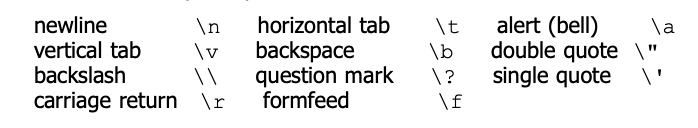
\includegraphics[width=0.7\textwidth]{img/C++中的转移序列.png}
\end{center}

\item 指定字面值的类型
\label{sec:org9a230d1}

通过添加下表中所列的前缀和后缀, 可以改变整型, 浮点型和字符型字面值的默认类型.

\begin{center}
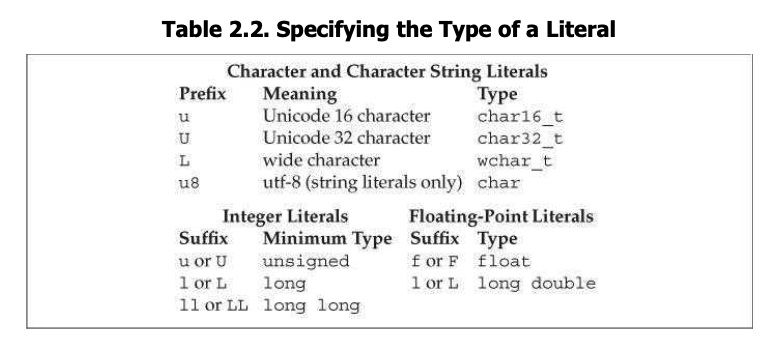
\includegraphics[width=0.7\textwidth]{img/指定字面值的类型.png}
\end{center}

下面是一些例子:

\begin{minted}[]{cpp}
L'a'    // 宽字符型字面值, 类型是 wchar_t
u8"hi!" // utf-8 字符串字面值
42ULL // 无符号整型字面值, 类型是 unsigned long long
1E-3F // 单精度浮点型字面值, 类型是 float
3.14159L // 拓展精度浮点型字面值, 类型是 long double
\end{minted}

\begin{note}
当使用一个长整型字面值时, 请使用大写字母 L 来标记, 因为小写字母 l 和数字 1 太容易混淆了.
\end{note}

\item 布尔字面值和指针字面值
\label{sec:orge49039c}

\texttt{true} 和 \texttt{false} 是布尔类型的字面值.

\texttt{nulptr} 是指针类型的字面值.
\end{enumerate}

\section{变量}
\label{sec:org3b356e7}

变量提供了一个具名的, 可供程序操作的存储空间. C++ 中的每个变量都有其数据类型, 数
据类型决定着变量所占内存空间的大小和布局方式, 该空间能储存的值的范围, 以及变量能
参与的运算. 对 C++ 程序员来说, ``变量(variable)'' 和 ``对象(object)'' 一般可以互换使
用.

\subsection{变量定义}
\label{sec:org6fff092}

变量定义的基本形式是: 首先是 \textbf{类型说明符} (type specifier), 随后紧跟由一个或多个
变量名组成的列表, 其中变量名以逗号分隔, 最后以分号结束.

如下所示:

\begin{minted}[]{cpp}
int usm = 0, value,
  unite_sold = 0;
Sales_item item;
std::string book("0-201-78345-X");
\end{minted}

\texttt{string} 和 \texttt{iostream} 一样是一种库类型, 是一种表示可变长字符序列的数据类型.

\begin{definition}[何为对象]
C++ 程序员们在很多场合都会使用 对象(object) 这个名词. 通常情况下, 对象是指一块存储数据并具有某种类型的内存空间.

本书中使用对象这个词时, 并不严格区分是类还是内置类型, 也不区分是否命名或是否只读.
\end{definition}

\begin{enumerate}
\item 初始值
\label{sec:orgd7b6201}

当对象在创建时获得了一个特定的值, 我们说这个对象被 \textbf{初始化} (initialized) 了.

当一次定义了两个或多个变量时, 对象的名字随着定义也就马上可以使用了. 因此我们可以
使用先定义的变量值去初始化后定义的其他变量. 如下所示:

\begin{minted}[]{cpp}
double price = 109.99, discount = price * 0.16;

double salePrice = applyDiscount(price, discount);
\end{minted}

很多程序员对于使用 \textbf{等号} (=) 来初始化变量的方式感到困惑, 这种方式容易让人认为初始
化时 \textbf{赋值} 的一种. 事实上, C++语言中, 初始化和赋值是两种完全不同的操作.

\vspace*{1\baselineskip}
\begin{note}
初始化不是赋值, 初始化的含义是创建变量时赋予其一个初始值, 而赋值的含义是把对象的当前值擦除, 而以一个新值来替代.
\end{note}

\item 列表初始化
\label{sec:org6033b84}

C++定义了好几种不同形式的初始化语句.

下面是一个例子:

\begin{minted}[]{cpp}
int units_sold = 0;
int unite_sold = {0};
int units_sold{0};
int units_sold(0);
\end{minted}

作为 C++11 新标准的一部分, 用花括号来初始化变量得到了全面应用.

这种初始化被称为 \textbf{列表初始化} (list initialization).

当用于内置类型的变量时, 这种初始化形式有一个重要特点: 如果我们使用列表初始化且初
始值存在丢失信息的风险, 则编译器会报错:

\begin{minted}[]{cpp}
long double ld = 3.1415926536;
int a{ld}, b = {ld}; // 错误: 转换未执行, 因为存在丢失信息的危险
int c(ld), d = ld;   // 正确: 转换执行, 确实丢失了部分值
\end{minted}

\item 默认初始化
\label{sec:orgacafbfa}

如果定义变量时没有指定初值, 则变量被 \textbf{默认初始化} (default initialized), 此时变
量被赋予了默认值, 默认值由变量类型决定.

如果是内置类型的变量未被显示初始化, 它的值由定义的位置决定. 定义于任何函数体之外
的变量被初始化为 0. 定义于函数体内部的内置类型将 \textbf{不被初始化} (uninitialized).

一个未被初始化的内置类型变量的值是未定义的, 如果试图拷贝或以其他形式访问此类值将
会出错.

每个类各自决定其初始化对象的方式. 而且, 是否允许不经初始化就定义对象也由类自己决
定. 如果类允许这种行为, 他将决定对象的初始值到底是什么.

\vspace*{1\baselineskip}
\begin{note}
定义于函数体内的内置类型的对象如果没有初始化, 则其值未定义. 类的对象如果没有显示地初始化, 则其值由类确定.
\end{note}
\end{enumerate}

\subsection{变量声明和定义的关系}
\label{sec:org2467baa}

为了允许把程序拆分成多个逻辑部分来编写, C++ 语言支持 \textbf{分离式编译} (separate
compilation) 机制, 该机制允许将程序分割成若干个文件, 每个文件可被独立编译.

如果将程序分为多个文件, 则需要有在文件之间共享代码的方法.

为了支持分离式编译, C++语言将声明和定义区分开来. \textbf{声明} (declaration) 使得名字为
程序所知, 一个文件如果想使用别处定义的名字则必须包含对那个名字的声明. 而 \textbf{定义}
(definition) 负责创建于名字关联的实体.

如果想声明一个变量而非定义它, 就在变量名前添加关键字 \texttt{extern}, 而且不要显示地初
始化变量:

\begin{minted}[]{cpp}
extern int i; // 声明 i 而非定义 i
int j;        // 声明并定义 j
\end{minted}

我们可以个由 \texttt{extern} 标记的变量赋予一个初始值, 但是这么做就抵消了 \texttt{extern} 的作
用.

\begin{minted}[]{cpp}
extern double pi = 3.1416; // 定义
\end{minted}

\vspace*{1\baselineskip}
\begin{note}
变量能且只能被定义一次, 但是可以被多次声明.
\end{note}

如果在多个文件中使用同一个变量, 就必须将声明和定义分离. 此时, 变量的定义必须出现
在且只能出现在一个文件中, 其他使用到该变量的文件必须对其进行声明.

\begin{definition}[静态类型]
C++ 是一种静态类型 (statically typed) 语言, 其含义是在编译阶段检查类型.
其中检查类型的过程被称为 类型检查(type checking).
\end{definition}

\subsection{标识符}
\label{sec:org256e18e}

C++ 的标识符(identifier) 是由字符, 数字和下划线组成, 其中必须以字母或下划线开头.
便是福的长度没有限制, 但是对大小写敏感.

\begin{enumerate}
\item 变量命名规范
\label{sec:org667ce03}

\begin{itemize}
\item 标识符要能体现实际含义
\item 变量名一般用小写字母, 如 \texttt{index}
\item 用户自定义的类名一般用大写字母开头, 如 \texttt{Sales\_item}.
\item 如果标识符由多个单词组成, 则单词间应该有明显区分.
\end{itemize}

\vspace*{1\baselineskip}
\begin{note}
对于命名规范来说, 若能坚持, 必将有效.
\end{note}

\begin{center}
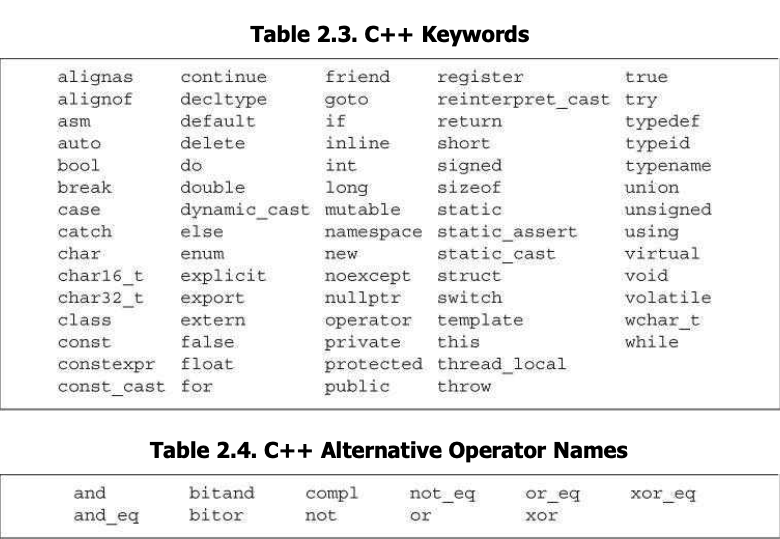
\includegraphics[width=0.7\textwidth]{img/C++ 关键字与操作符替代名.png}
\end{center}
\end{enumerate}
\end{document}
